\documentclass[11pt]{article}
\usepackage[a4paper,top=3cm,bottom=3cm,left=2.5cm,right=2.5cm]{geometry}
\usepackage[italian]{babel}
\usepackage[utf8x]{inputenc}
\usepackage {caption}
\usepackage {url}
\usepackage {multirow}
\usepackage {booktabs}
\usepackage {fixltx2e}
\usepackage {float}
\usepackage {graphicx}
\usepackage {cite}
\usepackage {listings}
\usepackage {color}
\usepackage {xcolor,colortbl}
\usepackage {adjustbox}
\usepackage {array}
\usepackage {svg}
\usepackage {subfig}
\usepackage {amssymb}
\usepackage {hyperref}
\usepackage {tabulary}
\usepackage {tabularx}
\usepackage[T1]{fontenc}
\usepackage{wasysym}
\usepackage{enumitem}
\usepackage{lipsum}

\newcommand{\voceU}[1]{%
	\item #1\dotfill\Square%
}

\newcommand{\voceD}[1]{%
	\item #1\hfill\Square%
}
\hypersetup{colorlinks=true,citecolor=black,linkcolor=black, urlcolor=blue}

\date{}

\renewcommand{\lstlistingname}{Listato}


\lstset{
    language=C,
    basicstyle=\ttfamily,
    breaklines=true,
    frame=single, % draw a frame at the top and bottom of the code block
    tabsize=2, % tab space width
    showstringspaces=false, % don't mark spaces in strings
    numbers=left, % display line numbers on the left
    captionpos=b,
    commentstyle=\color{green}, % comment color
    keywordstyle=\color{blue}, % keyword color
    stringstyle=\color{red} % string color
}

\begin{document}

\title{\textbf{Definizione ed Implementazione di un Sistema di Raccomandazione Distribuito per film
		e Modellazione di Eventi Complessi}}

\author{\\\textit{Prof. Ing.} Tommaso di Noia\\\textit{Prof.ssa} Marina Mongiello \\
	Mauro Losciale\\ 
	Pietro Tedeschi\\}

\clearpage\maketitle
\thispagestyle{empty}

\begin{center}
	
\includegraphics[scale=0.40]{images/poliba.jpg}
\end{center}

{\textbf{\center Logica e Intelligenza Artificiale\\Ingegneria del Software Avanzata\\ Laurea Magistrale in Ingegneria Informatica\\Politecnico di Bari\\A.A 2015 - 2016\\}}

\newpage
\clearpage
\thispagestyle{empty}
\renewcommand\contentsname{Indice}
\tableofcontents
\newpage
\setcounter{page}{1}

\newpage
\section{Introduzione}
\section{Stato dell'arte}

\subsection{Introduzione ai sistemi CEP}
L'incremento dei dispositivi interconnessi e delle applicazioni distribuite, richiede un'elaborazione continua del flusso dati. Esempi di tali applicazioni, vanno dal traffico generato dalle Wireless Sensor Networks (WSN) al flusso dati relativo agli indici finanziari, dal monitoraggio stradale alla Clickstream Analysis. 

Un sistema ad eventi complessi, meglio conosciuto come \textit{Complex Event Processing} (CEP), modella il flusso informativo dei dati, visualizzando gli elementi come notifiche di ciò che sta accadendo nel mondo esterno. I dati vengono rilevati e filtrati utilizzando dei pattern (oppure le \textit{processing rules}), i quali hanno il compito di rappresentare il modello di riferimento con l'informazione da rilevare, per poi farla pervenire alle rispettive parti (ad esempio, i dispositivi che effettuano una sottoscrizione ad un determinato topic nel paradigma \textit{publish-subscribe}). L'obiettivo di un sistema CEP consiste nell'identificare eventi significanti e rispondere ad essi nel più breve tempo possibile.
Un pattern o una regola, può essere definita mediante un linguaggio basato su query, il cosiddetto \textbf{Event Query
	Language}.
\begin{figure}[H]
	\centering
	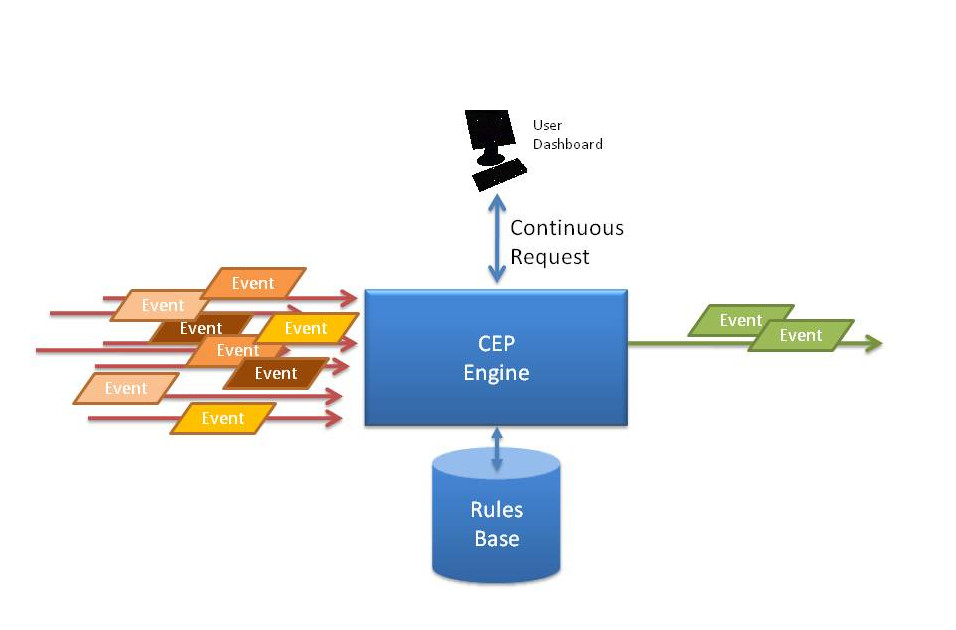
\includegraphics[scale=0.50]{images/CEP2.jpg}
	\caption{Architettura di un Sistema CEP\cite{cepimage}}
	\label{archcep}
\end{figure}

Gli \textbf{Event Query Languages} possono essere raggruppati in tre categorie: Composition Operators, Data Stream Query Languages e
Production Rules. I Composition Operators identificano gli eventi complessi partendo dalla composizione dei singoli eventi, utilizzando operatori quali congiunzione, negazione o di sequenza per la costruzione delle espressioni. Esempi rilevanti sono IBM Active Middleware Technology e ruleCore. 

I \textbf{Data Stream Query Languages} sono basati sul linguaggio SQL; gli stream di dati sono semplicemente tuple convertite per database relazionali, in modo che si possano eseguire query SQL su di esse. E' utile citare i seguenti approcci: CQL, Coral8, StreamBase,
Aleri, Esper e così via.

Le \textbf{Production Rules} specificano le azioni che devono essere eseguite quando il sistema si trova in determinati stati; non è un linguaggio ad eventi, ma costituisce un approccio importante nei sistemi CEP. Un esempio pratico è TIBCO Business Events.

Un altro fattore importante è il tempo. Sono due le parti da considerare quando si parla del tempo, il tempo della finestra ed il tempo dell'evento informativo. Il tempo della finestra mostra gli eventi che vengono esaminati in un determinato intervallo. Il tempo dell'evento invece, porta con se informazioni relative alla data, ora di rilevazione, tempo di transizione, ed intervallo di elaborazione.

I contributi relativi ai sistemi CEP, arrivano da diverse comunità, a partire da quelle che si occupano di sistemi distribuiti, automazione industriale, sistemi di controllo, monitoraggio delle reti, Internet of Things, e middleware in generale.

\begin{figure}[H]
	\centering
	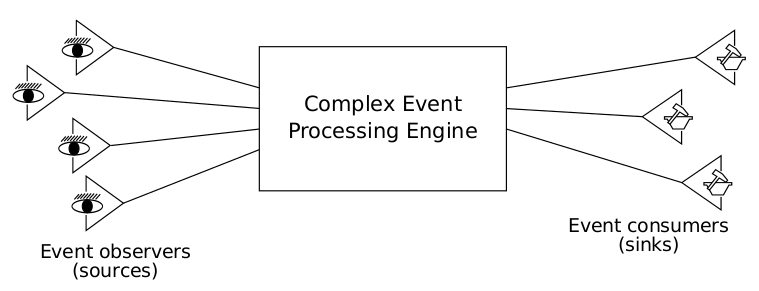
\includegraphics[scale=0.40]{images/CEP.png}
	\caption{Funzionamento di un Sistema CEP (High-Level) \cite{Cugola:2012:PFI:2187671.2187677}}
	\label{funcep}
\end{figure}

Come possiamo vedere dalla Figura \ref{funcep}, viene associata una semantica dettagliata agli elementi informativi da processare. Da una parte abbiamo gli \textbf{Event Observer}, i quali rappresentano la sorgente dei dati e degli eventi da notificare; in seguito abbiamo il \textbf{CEP Engine}, responsabile del filtraggio e della notifica degli eventi ai nodi \textit{sink}, identificati come \textbf{Event Consumers} \cite{Cugola:2012:PFI:2187671.2187677,fulop2010survey}.

\subsection{Sistemi di Raccomandazione}
I sistemi di raccomandazione, raccolgono informazioni sulle preferenze di utente in corrispondenza di un insieme di elementi (ad esempio, film, musica, libri, giochi, viaggi, siti web, applicazioni, gadget). L'informazione può essere acquisita in maniera esplicita (tipicamente ciò viene fatto acquisendo il voto di un utente) o implicitamente (analizzando il comportamento dell'utente, ad esempio musica ascoltata, applicazioni scaricate, siti web visitati, libri letti). Inoltre i sistemi di raccomandazione, possono tener conto anche delle caratteristiche demografiche dell'utente (ad esempio età, nazionalità, sesso); dei contenuti informativi presenti nel mondo del Web 2.0, ad esempio all'interno delle piattaforme di Social Networking, quali follower, followed, twit, like, post; dei dati provenienti dai dispositivi caratterizzanti l'Internet of Things (ad esempio, coordinate GPS, RFID, segnali medici inviati in real-time). 

I sistemi di raccomandazione utilizzano diverse sorgenti informative al fine di fornire all'utente finale una migliore Quality of Experience relativa alla predizione ed alla raccomandazione degli elementi che potrebbero interessargli. La tecnica del Collaborative Filtering (CF), ha un ruolo fondamentale nella raccomandazione, sebbene viene spesso usata anche con altre tecniche di filtraggio basate sul contenuto o basate sulla conoscenza. Il CF si basa sulla cronologia decisionale dell'utente: oltre alle nostre esperienze, facciamo le nostre decisioni anche in base alla conoscenza che ci circonda.

Il processo con cui un sistema di raccomandazione generi una raccomandazione, è basato sulla combinazione delle seguenti considerazioni:

\begin{enumerate}
\item La tipologia di dati disponibili nel databse (votazioni, informazioni di registrazione dell'utente, caratteristiche peculiari del contenuto informativo, relazioni sociali)
\item L'algoritmo di filtraggio usato (demografico, basato sul contenuto, collaborativo, basato sulle relazioni sociali, dipendente dal contesto e ibrido).
\item Il modello scelto (basato sull'uso diretto dei dati: 'memory-based', oppure un modello generato usando tali dati: 'model-based').
\item Le tecniche impiegate: approccio probabilistico, reti Bayesiane, algoritmi di tipo nearest neighbors, algoritmi genetici, reti neurali, logica fuzzy.
\item Livello di dispersione del database e scalabilità desiderata.
\item Capacità di elaborazione del sistema (tempo di elaborazione e consumi di memoria).
\item L'obiettivo da raggiungere (predizioni e raccomandazioni)
\item La qualità del risultato desiderata (ad esempio la precisione).
\end{enumerate}

La ricerca nell'ambito dei sistemi di raccomandazione, richiede che i dati siano di dominio pubblico, al fine di semplificare la ricerca sulle tecniche innovative relative all'analisi dei dati. Esempi di dataset pubblici presenti in letteratura, sono Last.Fm, Delicious, Netflix, MovieLens.
Le funzionalità interne per i sistemi di raccomandazione, sono caratterizzate dagli algoritmi di filtraggio. 
Gli algoritmi di filtraggio vengono classificati nel modo seguente:
\begin{enumerate}
	\item{a} Collaborative Filtering
	\item{b} Demographic Filtering
	\item{c} Content-Based Filtering
	\item{d} Hybrid Filtering
\end{enumerate}

Il \textbf{Content-Based Filtering} consente di creare raccomandazioni basate sulle scelte fatte in passato da un utente (ad esempio, in un sito E-Commerce, se l'utente ha acquistato una fiction cinematografica, probabilmente il sistema di raccomandazione gli consiglierà una fiction recente, che non ha ancora acquistato sul sito). La tecnica consente inoltre di generare la raccomandazione utilizzando il contenuto dell'oggetto, ad esempio il testo, le immagini, l'audio.

Il \textbf{Demographic Filtering} si basa sul principio che gli individui con caratteristiche personali comuni, quali età, sesso, luogo di residenza e così via, avranno le stesse preferenze.

Il \textbf{Collaborative Filtering} consente agli utenti di attribuire un voto ad un insieme di elementi (filmati, canzoni, film, libri, all'interno di una piattaforma web) salvando le proprie preferenze all'interno di un database, e consentendo di creare una raccomandazione specifica per ogni utente. I voti degli utenti possono essere anche acquisiti in maniera implicita (ad esempio il numero delle che viene ascoltata una canzone, il numero delle consultazioni relative ad una risorsa). L'algoritmo utilizzato maggiormente per il Collaborative Filtering è il $k$ Nearest Neighbors ($k$NN). 

Nella versione "\textit{user to user}", il KNN esegue i seguenti task per generare la raccomandazione:
\begin{enumerate}
\item Determinare i $k$ utenti vicini, per l'utente corrente.
\item Implementare un approccio 
\item Estrarre le predizioni dal passo 2 e selezionare le $N$ raccomandazioni.
\end{enumerate}

(1) determine k users neighbors (neighbor-hood) for the active user a; (2) implement an aggregation approach with the ratings for the neighborhood in items not rated by a; and (3) extract the predictions from in step 2 then select the top N
recommendations.

Hybrid filtering [47,185]. Commonly uses a combination of CF with demographic filtering [224] or CF with content-based filtering [18,60] to exploit merits of each one of these techniques. Hybrid filtering is usually based on bioinspired or probabilistic methods
such as genetic algorithms [76,99], fuzzy genetic [7], neural networks [133,62,192], Bayesian networks [50], clustering [209] and latent features [199].

A widely accepted taxonomy divides recommendation methods into memory-based and model-based method categories:
Memory-based methods [3,51,123,214]. Memory-based methods
can be defined as methods that (a) act only on the matrix of user
ratings for items and (b) use any rating generated before the refer-
ral process (i.e., its results are always updated). Memory-based
methods usually use similarity metrics to obtain the distance be-
tween two users, or two items, based on each of their ratios.
Model-based methods [3,212]. Use RS information to create a
model that generates the recommendations. Herein, we consider
a method model-based if new information from any user outdates
the model. Among the most widely used models we have Bayesian
classifiers [59], neural networks [107], fuzzy systems [234], genetic
algorithms [76,99], latent features [251] and matrix factorization
[142], among others.

To reduce the problems from high levels of sparsity in RS dat-
abases, certain studies have used dimensionality reduction tech-
niques [202]. The reduction methods are based on Matrix
Factorization [124,142,143]. Matrix factorization is especially ade-
quate for processing large RS databases and providing scalable ap-
proaches [215]. The model-based technique Latent Semantic Index
(LSI) and the reduction method Singular Value Decomposition
(SVD) are typically combined [224,244,48]. SVD methods provide
good prediction results but are computationally very expensive;
they can only be deployed in static off-line settings where the
known preference information does not change with time.

RS can use clustering techniques to improve the prediction qual-
ity and reduce the cold-start problem when applied to hybrid fil-
tering. It is typical to form clusters of items in hybrid RS
[209,237]. A different common approach uses clustering both for
items and users (bi-clustering) [252,85]. RS comprising social infor-
mation have been clustered to improve the following areas: tagging
[208], explicit social links [179] and explicit trust information
[181,70].

The graph in Fig. 3 shows the most significant traditional meth-
ods, techniques and algorithms for the recommendation process as
well as their relationships and groupings. Different sections of this
paper provide more detail on the most important aspects involved
in the recommendation process.

As may be seen in Fig. 3, we can use some of the traditional fil-
tering methods (content-based, demographic and collaborative)
applied to databases. Model-based technologies (genetic algo-
rithms, neural networks, etc.) make use of this kind of information.
Typical memory-based approaches are: item to item; user to user;
and hybrids of the two previous. The main purpose of both mem-
ory-based and model-based approaches is to get the most accurate
predictions in the tastes of users. The accuracy of these predictions
may be evaluated through the classical information retrieval mea-
sures, like MAE, precision, and recall.

VALUTAZIONE DEI SISTEMI DI RACCOMANDAZIONE
Since RS research began, evaluation of predictions and recom-
mendations has become important [94,201]. Research in the RS
field requires quality measures and evaluation metrics [90] to know
the quality of the techniques, methods, and algorithms for predic-
tions and recommendations. Evaluation metrics [94,95] and evalua-
tion frameworks [92,32] facilitate comparisons of several solutions
for the same problem and selection from different promising lines
of research that generate better results.
Because of evaluation measures, RS recommendations have
gradually been tested and improved [48]. A representative set of
existing evaluation measures has standard formulations, and a
group of open RS public databases has been generated. These two
advances have facilitated quality comparisons for new proposed
recommendation methods and previously published methods; thus,
RS methods and algorithms research has progressed continuously.
The most commonly used quality measures are the following
[90,95]: (1) prediction evaluations, (2) evaluations for recommen-
dation as sets, and (3) evaluations for recommendations as ranked
lists. Fig. 5 shows results from applying several evaluation mea-
sures to a set of representative similarity measures.
Evaluation metrics [12] can be classified as [94,95] (a) predic-
tion metrics: such as the accuracy ones: Mean Absolute Error
(MAE), Root of Mean Square Error (RMSE), Normalized Mean Average
Error (NMAE); and the coverage (b) set recommendation metrics:
such as Precision, Recall and Receiver Operating Characteristic
(ROC) [204] (c) rank recommendation metrics: such as the half-life
[43] and the discounted cumulative gain [17] and (d) diversity met-
rics: such as the diversity and the novelty of the recommended
items [105]. The validation process is performed by employing
the most common cross validation techniques (random sub-sam-
pling and k-fold cross validation) [21]; for cold-start situations,
due to the limited number of users (or items) votes involved, the
usual method chosen to carry out the experiments is leave-one-
out cross validation [36].
Hernández and Gaudioso [95] propose an evaluation process
based on the distinction between interactive and non-interactive subsystems. General publications and reviews also exist which in-
clude the most commonly accepted evaluation measures: mean
absolute error, coverage, precision, recall and derivatives of these:
mean squared error, normalized mean absolute error, ROC and fallout;
Goldberg et al. [87] focuses on the aspects not related to the eval-
uation, Breese et al. [43] compare the predictive accuracy of vari-
ous methods in a set of representative problem domains.
The majority of articles discuss attempted improvements to the
accuracy of RS results (RMSE, MAE, etc.). It is also common to at-
tempt an improvement in recommendations (precision, recall,
ROC, etc.). However, additional objectives should be considered
for generating greater user satisfaction [253], such as topic diversi-
fication and coverage serendipity.
Currently, the field has a growing interest in generating algo-
rithms with diverse and innovative recommendations, even at
the expense of accuracy and precision. To evaluate these aspects,
various metrics have been proposed to measure recommendation
novelty and diversity [105,220].
The frameworks aid in defining and standardizing the methods
and algorithms employed by RS as well as the mechanisms to eval-
uate the quality of the results. Among the most significant papers
that propose CF frameworks are Herlocker et al. [92] which
evaluates the following: similarity weight, significance weighting,
variance weighting, selecting neighborhood and rating normaliza-
tion; Hernández and Gaudioso [95] proposes a framework in which
any RS is formed by two different subsystems, one of them to
guide the user and the other to provide useful/interesting items.
Koutrika et al. [125] is a framework which introduces levels of
abstraction in CF process, making the modifications in the RS more
flexible. Antunes et al. [12] presents an evaluation framework
assuming that evaluation is an evolving process during the system
lifecicle.
The majority of RS evaluation frameworks proposed until now
present two deficiencies: the first of these is the lack of formal-
ization. Although the evaluation metrics are well defined, there
are a variety of details in the implementation of the methods
which, in the event they are not specified, can lead to the
generation of different results in similar experiments. The
second deficiency is the absence of standardization of the evalu-
ation measures in aspects such as novelty and trust of the
recommendations.
Bobadilla et al. [32] provides a complete series of mathematical
formalizations based on sets theory. Authors provide a set of eval-
uation measures, which include the quality analysis of the follow-
ing aspects: predictions, recommendations, novelty and trust.
Presented next is a representative selection of the RS evaluation
quality measures most often used in the bibliography. In order to measure the accuracy of the results of an RS, it is
usual to use the calculation of some of the most common predic-
tion error metrics, amongst which the Mean Absolute Error
(MAE) and its related metrics: mean squared error, root mean
squared error, and normalized mean absolute error stand out.

We define U as the set of the RS users, I as the set of the RS
items, r u,i the rating of user u on item i,  the lack of rating (r u,i = 
means user u has not rated item i), p u,i the prediction of item i on
user u.
Let O u = {i 2 Ijp u,i –  ^ r u,i – }, set of items rated by user u hav-
ing prediction values. We define the MAE and RMSE of the system
as the average of the user’s MAE. We remark that the absolute dif-
ference between prediction and real value, jp u,i  r u,i j, informs
about the error in the prediction. RMSE 1⁄4
ðp  r u;i Þ 2
#U u2U #O u i2O u;i
MAE 1⁄4
ð1Þ
ð2Þ
u
The coverage could be defined as the capacity of predicting from
a metric applied to a specific RS. In short, it calculates the percent-
age of situations in which at least one k-neighbor of each active
user can rate an item that has not been rated yet by that active
user. We defined K u,i as the set of neighbors of u which have rated
the item i.
\subsubsection{Filtro collaborativo}
\subsection{Introduzione allo Stream Processing}
\subsubsection{Il paradigma Publish-Subscribe}
\subsection{Il pattern Facade}
\subsection{Il pattern Singleton}
\subsection{Il pattern Model-View-Controller (MVC)}
\subsection{La tecnologia WebSocket}

\section{Analisi del progetto}

\section{Soluzione proposta}

\subsection{La libreria Spark}

Apache Spark è un sistema di cluster computing di tipo general-purpose, scalabile e veloce. Dispone di API di alto livello in \textbf{Java}, \textbf{Scala},\textbf{ Python} ed \textbf{R}, e un engine ottimizzato che supporta grafi di esecuzione generici. Supporta inoltre un ampio set di tool come \textbf{Spark SQL}, per structured data processing, \textbf{MLlib} per il machine learning e \textbf{Spark Streaming}, descritti nelle sezioni successive. Spark è eseguibile sia su sistemi Windows che UNIX-like (Linux, Mac OS). \\

Una delle possibili configurazioni di un sistema Spark è la modalità \textit{cluster}, mostrata in Figura \ref{spark-cluster}. 

\begin{figure}[H]
	\centering
	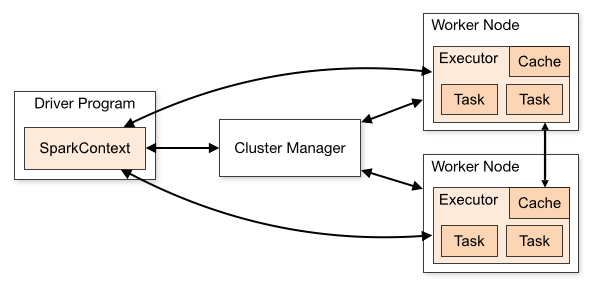
\includegraphics[scale=0.50]{images/cluster-overview.png}
	\caption{Configurazione in Spark di tipo Cluster Mode}
	\label{spark-cluster}
\end{figure}

Le applicazioni Spark sono eseguite come un set di processi indipendenti sul cluster, coordinati dall'oggetto \textit{SparkContext} del programma sorgente (detto \textbf{driver program}). Precisamente, il programma driver può connettersi su diversi tipi di \textit{cluster managers} (ad esempio un cluster di tipo Standalone, Mesos o YARN), il quale alloca le risorse a disposizione delle applicazioni. Una volta connesso, Spark scansiona i nodi del cluster alla ricerca degli \textbf{executor} (detti anche \textit{worker node}), i quali eseguono effettivamente i task e il data storage delle applicazioni. A questo punto il driver invia il codice dell'applicazione agli executor (tipicamente un file JAR o file Python incluso nello SparkContext) e schedula i task per l'esecuzione parallela. 

Alcune considerazioni riguardo tale architettura sono: 
\begin{itemize}
	\item Ogni applicazione gestisce i propri workers, i quali restano attivi durante tutto il ciclo di vita ed eseguono task multipli in thread multipli. Questo implica un isolamento tra le applicazioni, sia lato scheduling (ogni driver schedula i propri tasks) sia lato executor (tasks relativi ad applicazioni differenti risiedono in JVM differenti). Tuttavia ciò implica che non è possibile condividere nativamente i dati tra applicazioni diverse, a meno di utilizzare uno storage system esterno.
	\item Il driver deve poter gestire le connessioni con i workers durante l'intero ciclo di vita dell'applicazione. Per questo motivo dev'essere sempre garantita la visibilità a livello di rete tra driver e workers durante l'esecuzione.
	\item \`E necessario che driver e worker abbiano, a livello di rete, una distanza relativamente breve, preferibilmente nella stessa LAN, affinché lo scheduling sia rapidamente eseguito. 
\end{itemize}

Il principio di funzionamento di Spark si basa sostanzialmente sul concetto di \textit{Resilient Distributed Dataset} (\textbf{RDD}). Un RDD è una collezione di dati su cui è possibile operare parallelamente, ed è distribuita su tutti i nodi del cluster come file system Hadoop oppure è generata da una collezione esistente in Java o Scala. \\

Una seconda astrazione è rappresentata dalle variabili condivise (\textit{shared variables}), utilizzate nelle computazioni parallele. Di default Spark tiene traccia delle variabili istanziate nei vari task, e consente se necessario di condividerle fra task o fra task e driver. Le variabili condivise possono essere di due tipi: di tipo \textit{broadcast}, il cui valore viene salvato nella cache per ogni nodo, e di tipo \textit{accumulatore}, per esempio contatori o sommatori.

\subsubsection{Spark Streaming}

Spark Streaming è un'estensione delle Core API di Spark per lo\textbf{ stream processing} di live data streams ad alto throughput. Supporta molteplici sorgenti di data stream come\textbf{ Kafka}, Flume, Twitter, ZeroMQ, Kinesis o socket TCP, i quali possono essere processati tramite direttive come \textit{map}, \textit{join}, \textit{reduce} e \textit{window}. Nel post processing è possibile salvare i data stream in un file system, in un database o visualizzarli in una live dashboard. Come ulteriore fase nella pipeline di operazione rientra anche il machine learning ed il graph processing. In Figura \ref{spark-streaming} viene riassunta l'architettura descritta. 

\begin{figure}[H]
	\centering
	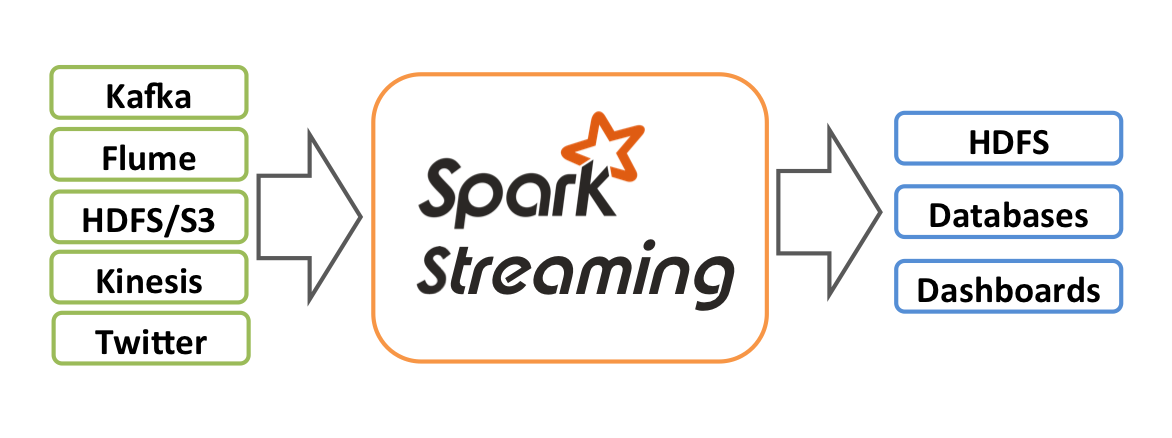
\includegraphics[scale=0.50]{images/streaming-arch.png}
	\caption{Architettura di Spark Streaming}
	\label{spark-streaming}
\end{figure}

Nello specifico, i data streams ricevuti vengono suddivisi in frammenti (\textit{batches}), processati da Spark per generare lo stream finale risultante in batches, come mostrato in Figura \ref{spark-streaming-processing}.

\begin{figure}[H]
	\centering
	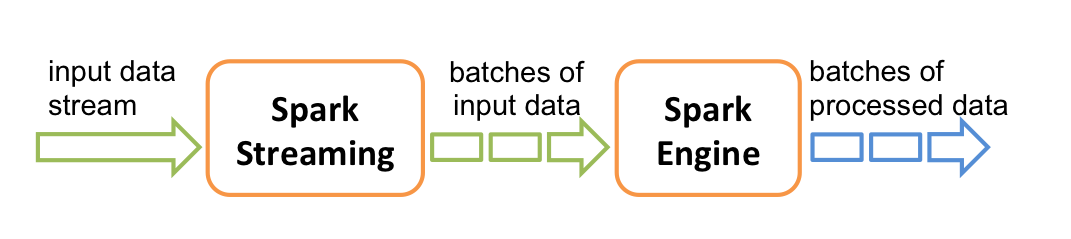
\includegraphics[scale=0.50]{images/streaming-flow.png}
	\caption{Spark Streaming Data Stream Processing}
	\label{spark-streaming-processing}
\end{figure}

A livello alto il flusso continuo di dati è rappresento da una struttura astratta detta \textit{discretized stream} o \textit{DStream}, il cui contenuto è rappresentato da tutte le sorgenti collegate eventualmente con Spark, o da stream risultati da altri DStream. Internamente, un DStream è rappresentato tramite una sequenza di RDD. 

\subsubsection{Spark MLlib}
\subsubsection{Spark SQL}

\subsection{Apache Kafka}
\subsubsection{Panoramica}
\subsubsection{Integrazione con Spark Streaming}

\subsection{Il framework Node.js}
\subsubsection{Panoramica}
\subsubsection{Kafka Client per Node.js}
\subsubsection{Il framework Angular.js}
\subsection{La libreria socket.IO}

\section{Conclusioni e sviluppi futuri}

\clearpage
\addcontentsline{toc}{section}{Bibliografia}
\nocite{*}
\bibliographystyle{plain}
\bibliography{biblib}


\end{document}